\documentclass[11pt, a4paper]{article} 
\usepackage[utf8]{inputenc}
\usepackage[nolist,nohyperlinks]{acronym}
\usepackage{geometry}
\usepackage{setspace}

\usepackage{biblatex}
\usepackage[hidelinks]{hyperref}
\usepackage{nameref}

\usepackage{graphicx}
\usepackage{float}
\usepackage[hypcap=false]{caption}
\usepackage{subcaption}

\usepackage{tabularx}
\usepackage{multirow}

\usepackage{lipsum}


\onehalfspacing
\addbibresource{arfeedback.bib}

% TabularX column defintions
\newcolumntype{L}[1]{>{\raggedright\let\newline\\\arraybackslash\hspace{0pt}}m{#1}}
\newcolumntype{C}[1]{>{\centering\let\newline\\\arraybackslash\hspace{0pt}}m{#1}}
\newcolumntype{R}[1]{>{\raggedleft\let\newline\\\arraybackslash\hspace{0pt}}m{#1}}

% Original assignment: Evaluate how to react on wrong AR usage
\newcommand{\mytitle}{Evaluation of Textual Feedback for Incorrect Usage of an Augmented Reality Application}
\newcommand{\runninghead}{Feedback for Augmented Reality}
\newcommand{\myauthor}{Julian Lüken, Mehmed Mustafa, Jan Schneider,\\ Steffen Tunkel, Chris Warin}
\newcommand{\myuni}{Georg-August University, Göttingen}
\newcommand{\titlespace}{1em}

% Header
\markright{\uppercase{\runninghead}\hfill}
\newenvironment{myabstract}{\begin{abstract}\begin{itshape}}{\end{itshape}\end{abstract}}

\begin{document}
	% Acronyms go here, refer to them with \ac{shorthand}
	\begin{acronym}
		\acro{AR}{Augmented Reality}
		\acro{SUS}{System Usability Scale}
	\end{acronym}

	\newgeometry{left=25mm,right=25mm,top=30mm,bottom=30mm}
	\pagestyle{empty}
	\begin{center}
		\begin{minipage}{.8\textwidth}
			\centering
			\begin{doublespace}\huge\textbf{\mytitle}\normalsize\\[\titlespace]\end{doublespace}
			\textsc{\myauthor}\\[\titlespace]
			\today\\[\titlespace]
			\myuni\\[\titlespace]
		\end{minipage}
	\end{center}
	\vspace{\titlespace}
	\begin{myabstract}
		% Abstract goes here
		\lipsum[1-3]
	\end{myabstract}
	\newgeometry{left=25mm,right=25mm,top=30mm,bottom=30mm}
	\pagestyle{myheadings}
	\pagebreak

	% REMEMBER
	%
	% Write in active, not passive
	% Write as "we"
	% Only two tenses (present and past)
	% Use LaTeX acronym environment (use \ac{shorthand} and define them right after \begin{document})
	% No paragraphs with only one sentence
	% No different types of paragraphs for pseudo-structuring
	% No forward references
	% Cite consistently and clearly (\cite{Lastname1999}, Jabref)
	% Footnotes: Just where really required
	% No repetitions

	\section*{Introduction}\label{sec:introduction}
		% Motivation
		% * Growing use of Augmented Reality and Lack of good feedback
		% * new technology: people don't yet know how to use AR features
		% * making AR usable without huge introductory efforts
		%
		% Research goals/questions
		% * To provide appropriate feedback to "wrong" AR usage/gestures
		% 	* To decide what type of feedback is better in comparison to other types
		%
		% Structure of report
		% * "For validation of our approach we conducted a usability case study"
		% * What will follow in the next sections
		%
		In recent years the number of available \ac{AR} applications has increased.
		Although \ac{AR} technology is no novelty, it was not widely available for society until a wide variety of smartphones were capable of running \ac{AR} applications.
		Since most users are newly discovering \ac{AR} technology, they don't know how to use its features yet, thus using unsupported gestures as input, which leads to frustration.
		Our main motivation for conducting this research is the lack of good feedback in case of incorrect usage, which could help a lot of users to avoid repeating common mistakes.
		Providing good feedback could also help teach users to control \ac{AR} applications without the need of a separate introduction.

		Our research goal is to provide appropriate feedback to unsupported gestures and decide what type of textual feedback is better in comparison to other types. For validation of our approach we conducted a usability case study.

		The organization of the paper is as follows. The section \nameref{sec:foundations} gives information about usability in general and the \ac{AR} environment we provide the feedback for. In the section \nameref{sec:relatedwork} we discuss similar work on \ac{AR} and feedback done in the past.
		The \nameref{sec:approach} section gives a detailed illustration of the feedback we present to users. In the section \nameref{sec:casestudy}, we talk about the setup case study we conducted in order to validate our approach, followed by our results and the discussion thereof. Lastly, we summarize and conclude in the \nameref{sec:summary}. 

	\section*{Foundations}\label{sec:foundations}
		% * What is AR?
		% * Which frameworks/technologies were used?
		% 	* Brief info about Vivian (which relies on state machines)
		% 		* What gestures are "correct"? (vivian relies on 1 finger shit and moving environment)
		%
		% * What is Usability(-testing)?
		% 	* Explain SUS (how did we tailor it to serve our purposes?)
		%
		% To move an object in Vivian-based apps, the user has to put his finger on the object, drag it, and let go of it in the desired spot. To cover greater distances, the user can move the device. Similarly, to rotate an object in Vivian, the user has to hold their finger on the object and rotate the device until they find the desired orientation.
		%
		Since one of the main goals of this study is to find suitable user feedback for augmented reality environments, it shall be further clarified what \ac{AR} means in the context of this study and which technologies were used during it. \ac{AR} itself is used to place 3D virtual objects into a 3D real environment in real time. In our study we used three different mobile phones which are running our applications. At runtime the recorded imagery of the phone is being augmented and shown to the user, to display a mix of virtual objects and the real world.

		For the design of the prototypes we used Unity3D as well as Blender. The functionalities of the prototypes have been implemented using the Vivian Framework which can be used to evaluate the usability of virtual prototypes. This is done by first modeling the virtual prototype and then modeling one or more state-machines to define the prototypes functionality.

		To evaluate the different types of feedback, we decided to use usability testing as a tool to quantify the corresponding results. Therefore we chose to have the users fill out a \ac{SUS} questionnaire which we tailored to fit our needs. The basic \ac{SUS} consists of ten questions regarding a systems usability. We added a few questions which target the feedback more as well as an open feedback field, where the participants are able to share their thoughts on the system with us.

		% graphics:
		% * all feedback message types in response to one gesture (i.e. pinch zoom) for all prototypes, i.e.
		%	* toaster front view type 1 "pinch zoom"
		%	* toaster rear view type 2 "pinch zoom"
		%	* microwave front view type 3 "pinch zoom"

		\begin{figure}[H]
			\centering
			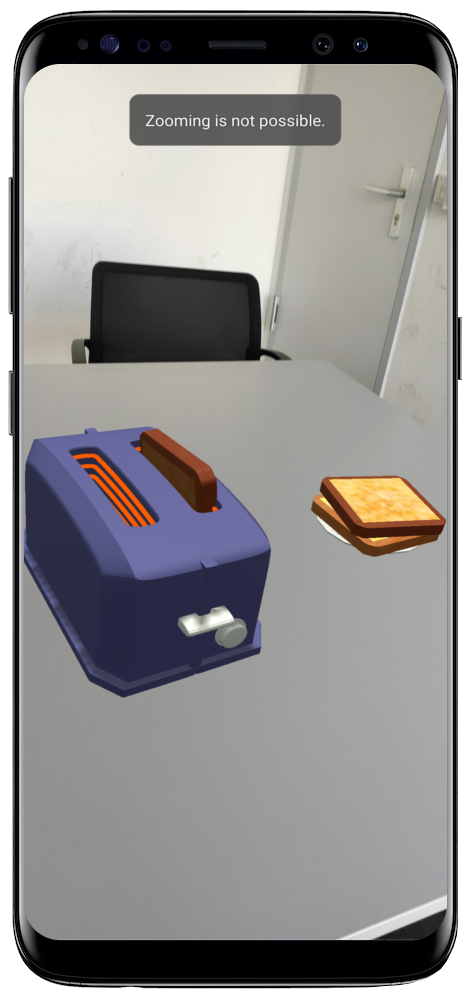
\includegraphics[width=.32\textwidth]{img/phone/phonepz1.png}
			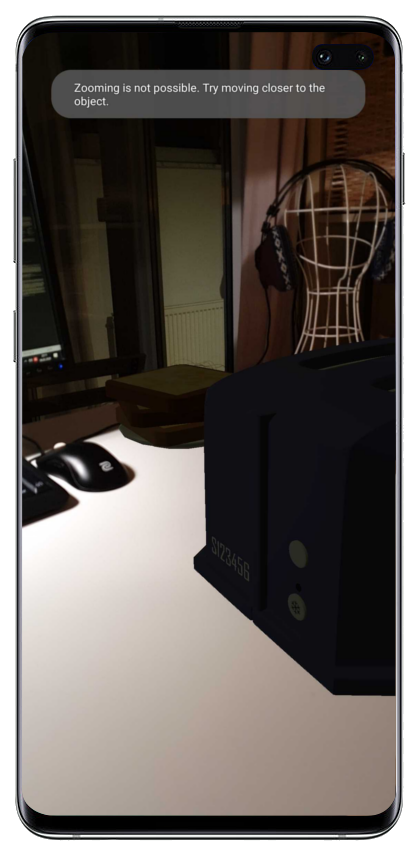
\includegraphics[width=.32\textwidth]{img/phone/phonepz2.png}
			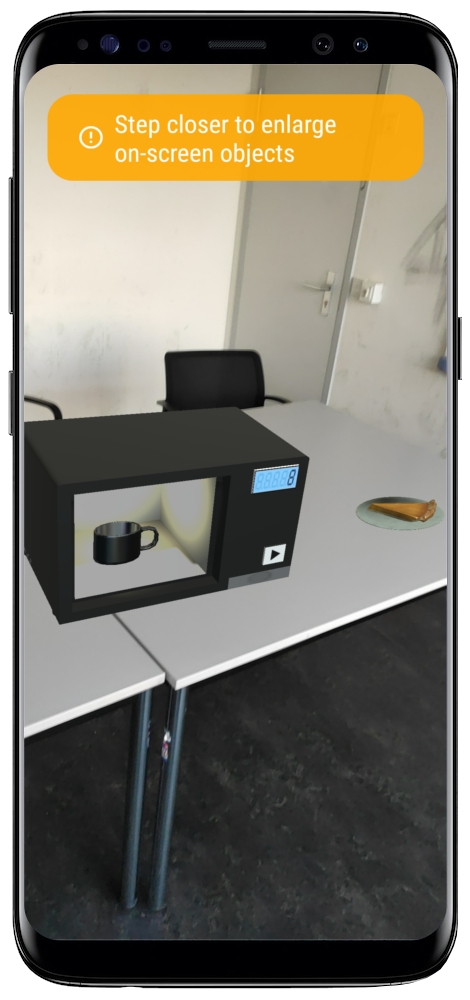
\includegraphics[width=.32\textwidth]{img/phone/phonepz3.png}
			\begin{subfigure}[t]{.32\textwidth}\centering
				\textbf{(A)}
			\end{subfigure}
			\begin{subfigure}[t]{.32\textwidth}\centering
				\textbf{(B)}
			\end{subfigure}
			\begin{subfigure}[t]{.32\textwidth}\centering
				\textbf{(C)}
			\end{subfigure}
			\caption{Three screenshots of an app made with the Vivian framework}
			\label{fig:feedbackonphone}
		\end{figure}

	\section*{Related Work}\label{sec:relatedwork}
		% Papers (as to be found in *.bib):
		% * Dey2016: A Systematic Review of 10 Years of Augmented Reality Usability Studies: 2005 to 2014
		% * Nilsson2007: Fun and Usable: Augmented Reality Instructions in a Hospital Setting
		% * Poupyrev2002: Developing a Generic Augmented Reality Interface
		%
		% parallels between above papers and this one
		% where do we come into play in above papers?
		% establish link between recent and past research
		%


	\section*{Approach}\label{sec:approach}
		% What are "wrong" inputs? Which ones are "wrong"?
		% Describe feedback messages (size, color, content, duration) for each implementation <- graphics
		% Why these messages?
		% maybe a nice reference table for that too
		In order to find feedback in response to incorrect usage of an \ac{AR} application, we have to define what kinds of gestures we consider incorrect in the first place. The user interface provided by the Vivian framework is based on one finger inputs (see \nameref{sec:foundations}), therefore we should take into consideration each input that is not done with a single finger. Prominent examples for multiple finger gestures are the \emph{pinch zoom} and the \emph{two finger rotation}. The pinch zoom is a gesture in which two fingers are placed on the touch screen and moved apart in opposite directions. The two finger rotation is a gesture in which two fingers are placed on the touch screen also and are together moved clockwise or counterclockwise about the center of the positions of the fingers. Common misconceptions by inexperienced \ac{AR} users might include using said pinch zoom to either zoom in on objects or to bring them closer, or using two finger rotation to rotate objects.

		To make users quickly and easily understand the controls of Vivian-based apps, we extended the Vivian framework to provide three feedback message implementations that differ in content, colors, size and duration. The content of the first feedback implementation is a \emph{critique}. If the user inputs a gesture that we consider incorrect, the app outputs a message that said input is not possible. For example, if a user tried pinch zooming, they would receive a message saying: "Pinch zooming is not possible". The content of the second feedback implementation is \emph{critique} and \emph{support}. The user is provided with a message stating that above mentioned input is not possible and hinting them towards what they should try instead. In the scope of the previous example, such a message would say: "Pinch zooming is not possible. Try moving around the object." In the first two implementations, the messages have the same size, color scheme and a duration of [X] seconds. The third implementation is more concise \emph{support}. For our previous example the exact message is saying: "Step closer to enlarge on-screen objects." It also differs in color scheme and size (see Figure \ref{fig:feedbackonphone}). It is displayed for [X] seconds.

		\begin{center}
			\begin{tabular}{|C{.05\textwidth}|L{.15\textwidth}|L{.23\textwidth}|L{.45\textwidth}|} \hline
										& \textbf{Description}												& \textbf{Gesture (input)} 					& \textbf{Response (output)} 											\\ \hline
				\multirow{2}{*}{\#1}	& \multirow{2}{*}{\parbox{.15\textwidth}{critique}}					& two finger rotation						& Rotating the object is not possible.									\\ \cline{3-4}
										& 																	& pinch zoom								& Zooming is not possible. 												\\ \hline
				\multirow{2}{*}{\#2}	& \multirow{2}{*}{\parbox{.15\textwidth}{combined}}					& two finger rotation						& Rotating the object is not possible. Try moving around the object.	\\ \cline{3-4}
										& 																	& pinch zoom								& Zooming is not possible. Try moving closer to the object.				\\ \hline
				\multirow{3}{*}{\#3}	& \multirow{3}{*}{\parbox{.15\textwidth}{support}}					& two finger rotation (movable object)		& Hold the phone and move the object to rotate							\\ \cline{3-4}
										& 																	& two finger rotation (elsewhere)			& Move around the objects												\\ \cline{3-4}
										&																	& pinch zoom 								& Step closer to enlarge on-screen objects								\\ \hline
			\end{tabular}
			\captionof{table}{The responses for each input in each implementation.}
			\label{tab:feedback}
		\end{center}

		The contents of each message can be found in Table \ref{tab:feedback}. The description column holds the names we assigned to the three different feedback implementations. In the gesture and response columns you can find the corresponding inputs and outputs respectively. If for example a user tried a two finger rotation, the app would display a message saying [X].
		In the support implemenentation we made the distinction between two finger rotations on movable objects and elsewhere. If the aforementioned center point of the two finger rotation is placed on a movable object (see \nameref{sec:foundations}), the app displays the message that corresponds to "two finger rotation (movable object)". If not, the "two finger rotation (elsewhere)" message is displayed.

	\section*{Case Study}\label{sec:casestudy}
		% SETUP
		% * introduce prototypes
		%	* functionalities
		%
		% * introduce groups(+subgroups)
		%	* size
		%	* what do they do
		%	* naming conventions
		%
		% * introduction to participants
		%
		% * tasks (hints)
		%
		% * what do we measure and how? 
		%	* screen recordings
		%	* notepad
		%
		% * questionnaire
		%	* SUS
		%	* open question
		%
		%
		% RESULTS
		% * first proto toaster
		% * first proto microwave
		% * second proto toaster
		% * second proto microwave
		%
		% * did wrong once vs did wrong multiple times
		%
		% * time to fulfill task per level
		% * time to fulfill tasks per prototype order
		% * number of wrong usages per level
		% * percentage of which group asking for more feedback
		% 
		% DISCUSSION
		% * hypothesis "visible and better feedback msg help the user to fulfill tasks faster, easier"
		% * feedback message must be genera enough to be applicable to any possible situation
		% * feedback message must be specific enough to be more helpful in the given situation
		% * outlines: sus/free answers
		% * easy prototype microwave -> intuitively usable, no feedback needed
		%
		% THREATS TO VALIDTY
		%
		\subsection*{Setup of the Case Study}\label{ssec:setup}
			To evaluate the quality of our feedback implementations we conducted a case study in the domain of usability engineering. We used two different prototypes supported by the Vivian Framework (see \nameref{sec:foundations}). Both of them are quite simple kitchen devices: a toaster prototype and a microwave prototype (as seen in Figure \ref{fig:feedbackonphone}).

			The microwave's functionality is limited to heating an object inside it with constant power. It has one button to add 10 seconds to the heating duration and one to open the door. The door can be closed by moving it. The status of the microwave is visually indicated by a small display showing the remaining heating time and a light inside the device, which turns on when it is open or heating. The toaster can toast one or two pieces of bread at a time. The toasting can be started by pulling down a handle and stopped by pushing it up again or by pressing the stop button, which is on the backside. Otherwise, the toasting stops automatically after a time which is defined by the position of a rotatable knob. The time mode is divided into 'low', 'medium' and 'high'. Further functionality is provided by the unfreezing mode, which can be activated by the snowflake button on the backside. The activation of the unfreezing mode results in a longer toasting duration and is indicated by a light above the button. The toasting process itself is displayed by the glowing of the heating elements. Both prototypes have a serial number on the backside. Both scenes contain different additional objects, which the user can interact with. These are pieces of bread for the toaster and for the microwave a cup which is already inside the microwave in the beginning and a piece of cake next to it.
			
			\begin{center}
				\begin{tabular}{|C{.05\textwidth}|L{.41\textwidth}|L{.41\textwidth}|}
					\hline \textbf{\#} & \textbf{Microwave} & \textbf{Toaster} \\
					\hline 1 & Read serial number off the microwave & Read serial number off the toaster \\
					\hline 2 & Heat up the cup & Toast the toast \\
					\hline 3 & Remove the cup, put the pie in, set the timer to 20 seconds and remove the plate at 5 seconds & Toast the toast on high heat and put the toaster in unfreezing mode \\
					\hline
				\end{tabular}
				\captionof{table}{The tasks for the different prototypes.}
				\label{tab:tasks}
			\end{center}

			Based on these functionalities we designed 3 tasks per prototype. As you can see on the concrete tasks in Table \ref{tab:tasks}, they are increasing in complexity. An example of this increase is that task 2 of the microwave asks to heat the cup, which is already in the microwave, for any time. Therefore just the start button has to be pressed once to fulfill the task. Afterwards, task 3 is to replace the cup by the pie and heat for a specific time. This contains a lot more necessary steps: open the door, move the cup out, move the pie in, close the door, press the start button multiple times and finally also press the stop button after the desired time is over.

			For the case study, we divided the participants into 4 groups. Each of these groups tested another version of the feedback implementation. Participants in group 0 got no feedback at all, in group 1 they got implementation 1, in group 2 implementation 2 and finally in group 3 implementation 3 (see \nameref{sec:approach}). We acquired 10 participants per group, so in total 40 people took part in the case study. Each participant was asked to fulfill the tasks for each prototype in the order provided in Table \ref{tab:tasks}. One half of the participants were asked to do the tasks of the toaster prototype first, while the other half did the tasks for the microwave prototype first. We were able to evaluate subgroups with a certain implementation level and a certain order of prototypes they tested. Each of those subgroups contained 5 participants. In the following, the subgroups are named \emph{TM}, which translates to "first toaster, then microwave" and \emph{MT}, which translates to "first microwave then toaster", followed by the number of their feedback group. For example, a participant who was assigned the toaster first and then the microwave without any feedback was in the subgroup TM0.

			Before the actual start of the test, we gave every participant a short introduction. This introduction contains information about the \ac{AR} technology and reasons behind usability testing to prepare the participants and create a similar level of expectation. It deliberately does not contain any information about how to use the application or the scope of the case study. This is important so the participants are not biased about wrong usage and the feedback they would get. During the test, we used screen recordings to measure each participants use of the application. These enabled us to acquire completion times for the different tasks and count the number of wrong usages. We used a notepad to register further observations.

			Following the test of the application the participants were asked to fill in a questionnaire. This questionnaire consists of 3 parts. First we asked participants if they have used \ac{AR} applications before. The second part is an \ac{SUS} (see \nameref{sec:foundations}) about the usability of the \ac{AR} application. The third part is an open question directly aimed to the feedback provided by the application, namely: "If you have any suggestions on what kind of feedback from the app you would find better, please let us know".

	\section*{Summary and Outlook}\label{sec:summary}
		\cite{Dey2016} \cite{Nilsson2007} \cite{Poupyrev2002} \ac{AR} \ac{AR}

	\pagebreak
	\printbibliography
\restoregeometry
\end{document}